\begin{figure}[htbp]
\centering
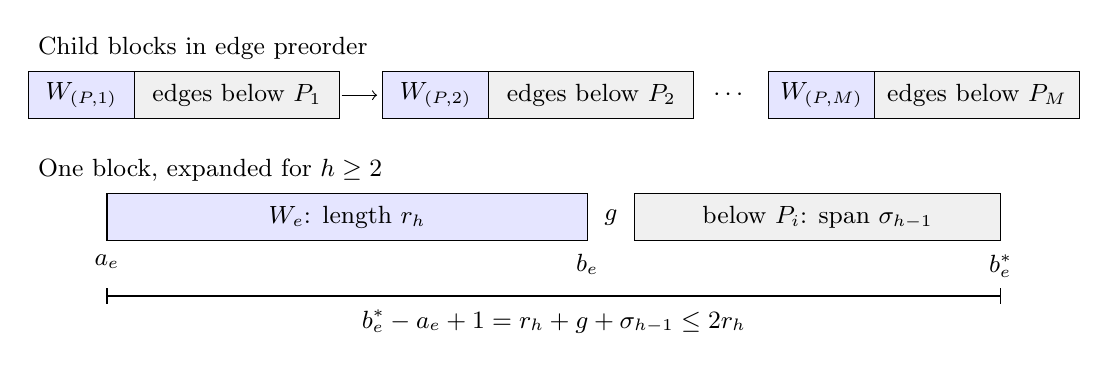
\begin{tikzpicture}[x=1cm,y=1cm,font=\small]
  \node[anchor=west] at (0,2.5) {Child blocks in edge preorder};
  \foreach \start/\index in {0/1,4.5/2,9.4/M}{
    \fill[blue!10] (\start,1.6) rectangle (\start+1.35,2.2);
    \fill[gray!12] (\start+1.35,1.6) rectangle (\start+3.95,2.2);
    \draw (\start,1.6) rectangle (\start+3.95,2.2);
    \draw (\start+1.35,1.6)--(\start+1.35,2.2);
    \node at (\start+.675,1.9) {$W_{(P,\index)}$};
    \node at (\start+2.65,1.9) {edges below $P_{\index}$};
  }
  \draw[->] (3.98,1.9)--(4.43,1.9);
  \node at (8.89,1.9) {$\cdots$};
  \node[anchor=west] at (0,.95) {One block, expanded for $h\ge2$};
  \fill[blue!10] (1,.05) rectangle (7.1,.65);
  \fill[gray!12] (7.7,.05) rectangle (12.35,.65);
  \draw (1,.05) rectangle (7.1,.65);
  \draw (7.7,.05) rectangle (12.35,.65);
  \node at (4.05,.35) {$W_e$: length $r_h$};
  \node at (7.4,.35) {$g$};
  \node at (10.025,.35) {below $P_i$: span $\sigma_{h-1}$};
  \node[anchor=north] at (1,0) {$a_e$};
  \node[anchor=north] at (7.1,0) {$b_e$};
  \node[anchor=north] at (12.35,0) {$b_e^*$};
  \draw (1,-.65)--(12.35,-.65);
  \draw (1,-.55)--(1,-.75);
  \draw (12.35,-.55)--(12.35,-.75);
  \node[anchor=north] at (6.675,-.7)
    {$b_e^*-a_e+1=r_h+g+\sigma_{h-1}\le2r_h$};
\end{tikzpicture}
\caption{Each edge window precedes the windows below its child, and
the child blocks are listed in order.  The lower diagram includes the
gap before a nonempty child subtree.  An edge into a leaf has no
following subtree or internal gap.  Lengths are schematic.}
\label{fig:windows}
\end{figure}
